\section{Introductory Ideas and Examples}
\begin{exercise} \label{ex:1-1}
    Find the ordinary power series generating functions of each of the following sequences, in simple, closed form. In each case the sequence is defined for all $n \geq 0$.
    \begin{enumerate}[label=(\alph*)]
        \item $a_n = n$
        \item $a_n = \alpha n + \beta$
        \item $a_n = n^2$
        \item $a_n = \alpha n^2 + \beta n + \gamma$
        \item $a_n = P(n)$, where $P(n)$ is a given polynomial, of degree $m$.
        \item $a_n = 3^n$
        \item $a_n= 5\cdot 7^n - 3\cdot 4^n$
    \end{enumerate}
\end{exercise}

\begin{solution}
    For each of the sequences, define $A(x) = \bsum a_n x^n$, then apply following steps.
    \begin{enumerate}
        \item Multiply both sides of the sequence definition by $x^n$ and sum over all $n \geq 0$.
        \item The left-hand side is recognized as $A(x)$.
        \item Express the right-hand side using known power series.
    \end{enumerate}

    \begin{enumerate}[label=(\alph*)]
        \item \hypertarget{eq:ch1:1:a}{} Apply $xD$ trick and bring the $xD$ outside.
            \[
                A(x) = \bsum n x^n \estep{\eqref{eq:xD}} \bsum xDx^n = xD\bsum x^n \overset{\eqref{eq:power_geom}}{=} xD\frac{1}{1-x} = \frac{x}{(1-x)^2}
            \] 
        \item \hypertarget{eq:ch1:1:b} Split the sum and handle each part separately.
            \[
                A(x) = \bsum \alpha n x^n + \bsum\beta x^n \estep{\hyperlink{eq:ch1:1:a}{1.1(a)},\eqref{eq:power_geom}} \frac{\alpha x}{(1-x)^2} + \frac{\beta}{1-x}
            \]
        \item Apply the $xD$ trick twice.
        \[
            A(x) = \bsum n^2x^n \estep{\eqref{eq:xD}} \bsum (xD)^2x^n \estep{\eqref{eq:power_geom}} (xD)^2 \frac{1}{1-x} = \frac{x+x^2}{(1-x)^3}
        \]
        \item A combination of the results from the previous parts.
        \[
            A(x) = \bsum \left(\alpha n^2 x^n + \beta n x^n + \gamma x^n \right) \estep{\hyperlink{eq:ch1:1:b}{1.1(b\text{-}c)}} \frac{\alpha x +\alpha x^2}{(1-x)^3} + \frac{\beta x}{(1-x)^2} + \frac{\gamma}{1-x}
        \]
        \item \hypertarget{eq:ch1:1:e} Let $P(n) = c_m n^m + c_{m-1} n^{m-1} + \ldots + c_1 n + c_0 $ and apply $xD$ trick multiple times.
        \begin{align*}
            A(x) &= \bsum \left(c_m n^m  + c_{m-1} n^{m-1}  + \ldots + c_1 n + c_0 \right)x^n \\
            \estepalign{\eqref{eq:xD}} (c_m (xD)^m + c_{m-1}(xD)^{m-1} + \ldots + c_0) \bsum x^n  \estep{\eqref{eq:power_geom}} P(xD) \frac{1}{1-x}
        \end{align*}
        \item
        \[
            A(x) = \bsum 3^n x^n = \bsum (3x)^n \estep{\eqref{eq:power_geom}} \frac{1}{1-3x}
        \]
        \item
        \[
            A(x) = 5\bsum (7x)^n - 3 \bsum (4x)^n \estep{\eqref{eq:power_geom}} \frac{5}{1-7x} - \frac{3}{1-4x}
        \]
    \end{enumerate}
\end{solution}

\begin{exercise} \label{ex:1-2}
    For each of the sequences given in Exercise~\ref{ex:1-1}, find the exponential generating function of the sequence in simple, closed form.
\end{exercise}
\begin{solution}
    For each of the sequences, define $A(x) = \bsum a_n \expcoeff$, then apply the method from the previous exercise but where $x^n$ is replaced by $\expcoeff$ in the first step.
    \begin{enumerate}[label=(\alph*)]
        \item \hypertarget{eq:ch1:2:a}
        \[
            A(x) = \bsum n\frac{x^n}{n!} \estep{\eqref{eq:xD}} \bsum xD \frac{x^n}{n!} = xD \bsum \frac{x^n}{n!} \estep{\eqref{eq:power_exp}} xD e^x = x e^x
        \]
        \item \hypertarget{eq:ch1:2:b} Split sum.
        \[
            A(x) = \bsum \alpha n \frac{x^n}{n!} + \bsum\beta \frac{x^n}{n!} \estep{\hyperlink{eq:ch1:2:a}{1.2(a)},\eqref{eq:power_exp}} \alpha x e^x + \beta e^x
        \]
        \item $xD$ trick twice.
        \[
            A(x) = \bsum n^2\frac{x^n}{n!} \estep{\eqref{eq:xD}} (xD)^2 \bsum \frac{x^n}{n!} \estep{\eqref{eq:power_exp}} (xD)(xe^x)= (x+x^2)e^x
        \]
        \item Combination of previous results.
        \[
            A(x) = \bsum \alpha n^2 \frac{x^n}{n!} + \beta n \frac{x^n}{n!} + \gamma \frac{x^n}{n!} \estep{\hyperlink{eq:ch1:2:b}{1.2(b\text{-}c)}}  \alpha (x + x^2)e^x + \beta xe^x + \gamma e^x
        \]
        \item Analogous to its Exercise~\ref{ex:1-1} counterpart.
        \[
            A(x) = (c_m(xD)^m + \ldots + c_1(xD) + c_0)\bsum \frac{x^n}{n!} \estep{\eqref{eq:power_exp}} P(xD)e^x
        \]
        \item
        \[
            A(x) = \bsum 3^n \frac{x^n}{n!} = \bsum \frac{(3x)^n}{n!} \estep{\eqref{eq:power_exp}} e^{3x}
        \]
        \item
        \[
            A(x) = 5\bsum \frac{(7x)^n}{n!} - 3 \bsum \frac{(4x)^n}{n!} \estep{\eqref{eq:power_exp}} 5e^{7x} - 3e^{4x}
        \]
    \end{enumerate}
\end{solution}

\begin{exercise}
    \label{ex:1-3}
    If $f(x)$ is the ordinary power series generating function of the sequence $\{a_n\}_{n\geq 0}$, then express simply, in terms of $f(x)$, the ordinary power series generating functions of the following sequences. In each case the range of $n$ is $0$, $1$, $2$, $\ldots$
    \begin{enumerate}[label=(\alph*)]
        \item $\{a_n + c\}$
        \item $\{\alpha a_n + c\}$
        \item $\{na_n\}$
        \item $\{P(n)a_n\}$, where $P$ is a given polynomial.
        \item $0, a_1, a_2, a_3, \ldots$
        \item $0, 0, 1, a_3, a_4, a_5, \ldots$
        \item $a_0, 0, a_2, 0, a_4, 0, a_6, 0, a_8, 0, \ldots$
        \item $a_1, a_2, a_3, \ldots$
        \item $\{a_{n+h}\}$ \quad ($h$ a given constant)
        \item $\{a_{n+2}+3a_{n+1}+a_n\}$
        \item $\{a_{n+2} - a_{n+1} - a_{n}\}$
    \end{enumerate}
\end{exercise}
\begin{solution}
    Let $g(x)$ be the ordinary power series of the desired sequences. The results follow from simple algebraic manipulations.
    \begin{enumerate}[label=(\alph*)]
        \item Split sum.
        \[
            g(x) =  \bsum (a_n + c) x^n= \bsum a_n x^n + c\bsum x^n \estep{\eqref{eq:power_geom}} f(x) + \frac{c}{1-x}
        \]
        \item Completely analogous as previous part.
        \[
            g(x) = \bsum (\alpha a_n +c) x^n = \alpha \bsum a_n x^n + c \bsum x^n \estep{\eqref{eq:power_geom}} \alpha f(x) + \frac{c}{1-x}
        \]
        \item \hypertarget{eq:ch1:3:c}{} $xD$ trick.
        \[
            g(x) = \bsum na_n x^n 
            \estep{\eqref{eq:xD}} xD \bsum a_n x^n 
             = xDf(x)
        \]
        \item \hypertarget{eq:ch1:3:d}{} Same method as \hyperlink{eq:ch1:1:e}{1.1(e)}.
        \[
            g(x) = \bsum (c_m (xD)^m + \ldots + c_1 (xD) + c_0)a_nx^n = P(xD)f(x)
        \]
        \item \hypertarget{eq:ch1:3:e} Add and subtract $a_0$ to become $f(x)$.
        \[
            g(x) = \sum_{n=1}^\infty a_n x^n =  -a_0 + \bsum a_n x^n = -a_0 + f(x) 
        \]
        \item Add and subtract $a_0 + a_1x + (a_2 - 1)x^2$.
        \[
            g(x) = -a_0 - a_1x - (a_2 - 1)x^2 + \bsum a_n x^n 
            = -a_0 - a_1x-(a_2-1)x^2 + f(x)
        \]
        \item \hypertarget{eq:ch1:3:g}{} Even part of $f(x)$.
        \begin{align*}
            g(x) &= \bsum a_{2n} x^{2n}
            = \frac{a_0}{2} + \frac{a_0}{2} + \frac{a_1}{2}x + \frac{a_1}{2}(-x) + \frac{a_2}{2}x^2+ \frac{a_2}{2}(-x)^2 + \ldots \\
            &= \bsum \frac{a_n}{2}x^n + \bsum \frac{a_n}{2} (-x)^n= \frac{f(x)}{2} + \frac{f(-x)}{2}
        \end{align*}
        \item \hypertarget{eq:ch1:3:h} Multiply and divide by $x$.
        \[
            g(x) = \bsum a_{n+1}x^n= \frac{\bsum a_{n+1}x^{n+1}}{x} =\frac{\sum_{n=1}^\infty a_nx^n}{x} \estep{\hyperlink{eq:ch1:3:e}{(e)}} \frac{-a_0 + f(x)}{x}
        \]
        \item \hypertarget{eq:ch1:3:i} Multiply and divide by $x^h$.
        \[
            g(x) = \bsum a_{n+h} x^n= \frac{\bsum a_{n+h}x^{n+h}}{x^h}= \frac{\sum_{n=h}^\infty a_{n}x^{n}}{x^h}
        \]
        Add and subtract $\sum_{n=0}^{h-1}a_nx^n$ in the numerator.
        \[
            g(x) = \frac{\bsum a_n x^n- \sum_{n=0}^{h-1} a_n x^n }{x^h}
             = \frac{f(x) - \sum_{n=0}^{h-1} a_n x^n}{x^h}
        \]
        \item The result follows from part \hyperlink{eq:ch1:3:i}{(i)} after splitting the sum.
        \begin{align*}
            g(x) &= \bsum a_{n+2}x^n + 3\bsum a_{n+1}x^n + \bsum a_n x^n  \\
            \estepalign{\hyperlink{eq:ch1:3:i}{1.3(i)}} \frac{f(x) - a_0 - a_1x}{x^2} + \frac{3f(x) - 3a_0}{x} + f(x)
        \end{align*}
        \item Completely analogous to the previous part.
        \begin{align*}
            g(x) &= \bsum a_{n+2}x^n - \bsum a_{n+1}x^n - \bsum a_n x^n \\
            \estepalign{\hyperlink{eq:ch1:3:i}{1.3(i)}} \frac{f(x) -a_0 - a_1x}{x^2} - \frac{f(x) - a_0}{x} - f(x)
        \end{align*}
    \end{enumerate}
\end{solution}

\begin{exercise} \label{ex:1-4}
    Let $f(x)$ be the \emph{exponential} generating function of a sequence $\{a_n\}$. For each of the sequences in Exercise \ref{ex:1-3}, find the exponential generating function simply, in terms of $f(x)$.
\end{exercise}
\begin{solution}
    The methodology and ideas are completely equivalent to the previous exercise. Let $g(x)$ be the exponential generating function of the desired sequence.
    \begin{enumerate}[label=(\alph*)]
        \item \[
            g(x) = \bsum (a_n + c) \frac{x^n}{n!} = \bsum a_n \frac{x^n}{n!} + c\bsum \frac{x^n}{n!} \estep{\eqref{eq:power_exp}} f(x) + ce^x
        \]
        \item \[
            g(x) = \bsum (\alpha a_n +c) \frac{x^n}{n!} = \alpha \bsum a_n \frac{x^n}{n!} + c\bsum \frac{x^n}{n!} \estep{\eqref{eq:power_exp}} \alpha f(x) + ce^x
        \]
        \item \[
            g(x) = \bsum na_n\frac{x^n}{n!} 
            \estep{\eqref{eq:xD}} (xD)\bsum a_n \frac{x^n}{n!}
            = xDf(x)
        \]
        \item \[
            g(x) = \bsum P(n) a_n \frac{x^n}{n!} \estep{\eqref{eq:xD}} P(xD) \bsum a_n \frac{x^n}{n!} = P(xD)f(x) 
        \]
        \item \hypertarget{eq:ch1:4:e} \[
            g(x) = \sum_{n=1}^\infty a_n \frac{x^n}{n!} = -a_0 + \bsum a_n \frac{x^n}{n!} = -a_0 + f(x)
        \]
        \item\[
            g(x) = \frac{x^2}{2!} + \sum_{n=3}^\infty a_n \frac{x^n}{n!} \\
            = -a_0 - a_1x - (a_2-1)\frac{x^2}{2} + f(x)
        \]
        \item \[
            g(x) = \bsum a_{2n} \frac{x^{2n}}{(2n)!} = \bsum \frac{a_n}{2} \frac{x^n}{n!} + \bsum \frac{a_n}{2} \frac{(-x)^n}{n!} = \frac{f(x)}{2} + \frac{f(-x)}{2}
        \]
        \item \hypertarget{eq:ch1:4:h}{} \[
                g(x) = \bsum a_{n+1}\frac{x^n}{n!}
            = \bsum a_{n+1} D\frac{x^{n+1}}{(n+1)!} =  D \sum_{n=1}^\infty a_n \frac{x^n}{n!}
            \]
            Now apply the result from part \hyperlink{eq:ch1:4:e}{(e)}.
            \[
                g(x) = D (-a_0 + f(x)) = Df(x) 
            \]
        \item \hypertarget{eq:ch1:4:i}{} \begin{align*}
            g(x) &= \bsum a_{n+h} \frac{x^n}{n!} = \bsum a_{n+h} D^h \frac{x^{n+h}}{(n+h)!} \\
            &= D^h \sum_{n=h}^\infty a_n \frac{x^n}{n!} = D^h \left(- \sum_{n=0}^{h-1} a_n\frac{x^n}{n!} + \bsum a_n \frac{x^n}{n!}\right)
        \end{align*}
            Because $D^h x^n = 0$ whenever $n < h$, we find:
            \[
                g(x) = D^h \bsum a_n \frac{x^n}{n!} = D^h f(x)
            \]
        \item Apply the result from part \hyperlink{eq:ch1:4:i}{(i)} of this exercise after splitting the sum.
        \begin{align*}
            g(x) &= \bsum a_{n+2}\frac{x^n}{n!} + 3 \bsum a_{n+1}\frac{x^n}{n!} + \bsum a_n \frac{x^n}{n!} \\
            \estepalign{\hyperlink{eq:ch1:4:i}{1.4(i)}} D^2f(x) + 3Df(x) + f(x)
        \end{align*}
        \item \begin{align*}
            g(x)
            &= \bsum a_{n+2}\frac{x^n}{n!} - \bsum a_{n+1}\frac{x^n}{n!} - \bsum a_n \frac{x^n}{n!} \\
            \estepalign{\hyperlink{eq:ch1:4:i}{1.4(i)}} D^2f(x) - Df(x) - f(x)
        \end{align*}
    \end{enumerate}
\end{solution}

\begin{exercise} \label{ex:1-5}
    Find 
    \begin{enumerate}[label=(\alph*)]
        \item $\coeff{x^n} e^{2x}$
        \item $\coeff{x^n/n!} e^{\alpha x}$ 
        \item $\coeff{x^n/n!} \sin x$
        \item $\coeff{x^n} \{1/((1-ax)(1-bx))\} \quad (a\neq b)$
        \item $\coeff{x^n}(1+x^2)^m$
    \end{enumerate}
\end{exercise}
\begin{solution}
    \begin{enumerate}[label=(\alph*)]
        \item \[
            \coeff{x^n}e^{2x} \estep{\eqref{eq:power_exp}} \coeff{x^n} \bsum[k] \frac{(2x)^k}{k!} = \coeff{x^n} \bsum[k] \frac{2^k}{k!}x^k = \frac{2^n}{n!}
        \]
        \item \[
            \coeff{\frac{x^n}{n!}}e^{\alpha x} \estep{\eqref{eq:power_exp}} \coeff{\frac{x^n}{n!}} \bsum[k] \frac{(\alpha x)^k}{k!} = \coeff{\frac{x^n}{n!}} \bsum[k] \alpha^k \frac{x^k}{k!} = \alpha^n
        \]
        \item
        \[
            \coeff{\frac{x^{n}}{n!}}\sin x \estep{\eqref{eq:power_sin}} \coeff{\frac{x^{n}}{n!}} \bsum[k] \frac{(-1)^k x^{2k+1}}{(2k+1)!} = \begin{cases}
                (-1)^{(n-1)/2} & \text{if $n$ is odd} \\
                0 & \text{otherwise}
            \end{cases}
        \]
        \item Apply partial fraction decomposition.
        \begin{align*}
            \coeff{x^n}\frac{1}{(1-ax)(1-bx)} &= \coeff{x^n} \frac{\frac{a}{a-b}}{1-ax} + \coeff{x^n}\frac{\frac{b}{b-a}}{1-bx} \\
            &= \frac{1}{a-b} \left(\coeff{x^n} \frac{a}{1-ax} - \coeff{x^n} \frac{b}{1-bx}\right) \\
            \estepalign{\eqref{eq:power_geom}} \frac{1}{a-b} \left(\coeff{x^n} a\bsum[k] (ax)^k - \coeff{x^n} b\bsum[k] (bx)^k \right) \\
            &= \frac{a^{n+1} - b^{n+1}}{a-b}
        \end{align*}
        \item
        \[
            \coeff{x^n}(1+x^2)^m \estep{\eqref{eq:binom_num}} \coeff{x^n} \infsum[k] \binom{m}{k} x^{2k} = \begin{cases}
                \tbinom{m}{n/2} & \text{if $n$ is even} \\
                0 & \text{otherwise}
            \end{cases}
        \]
    \end{enumerate}
\end{solution}

\begin{exercise}
    \label{ex:1-6}
    In each part, a sequence $\{a_n\}_{n\geq 0}$ satisfies the given recurrence relation. Find the ordinary power series generating function of the sequence.
    \begin{enumerate}[label=(\alph*)]
        \item $a_{n+1} = 3a_n + 2 \quad (n\geq 0;a_0=0)$
        \item $a_{n+1} = \alpha a_n + \beta \quad (n\geq 0;a_0=0)$
        \item $a_{n+2} = 2a_{n+1} - a_n \quad (n\geq 0; a_0=0; a_1=1)$
        \item $a_{n+1} = a_n / 3 +1 \quad (n \geq 0; a_0 = 0)$
    \end{enumerate}
\end{exercise}
\begin{solution}
    We use following method for all recurrences.
        \begin{enumerate}
            \item Define $f(x) = \bsum a_n x^n$.
            \item Multiply both sides by $x^n$ and sum over $n \geq 0$.
            \item Relate both sides to $f(x)$ (for example, using results from Exercise \ref{ex:1-3}).
            \item Solve for $f(x)$.
        \end{enumerate}
    \begin{enumerate}[label=(\alph*)]
        \item \[
            \bsum a_{n+1} x^n = \bsum 3a_n x^n + \bsum 2x^n
        \]
        With \hyperlink{eq:ch1:3:h}{1.3(h)} and \eqref{eq:power_geom}, we obtain
        \[
            \frac{f(x) - a_0}{x} = 3f(x) + \frac{2}{1-x} \overset{a_0=0}{\Longleftrightarrow}f(x) = \frac{2x}{(1-x)(1-3x)}
        \]
        \item \hypertarget{eq:ch1:6:b}{} Completely analogous as the previous part.
        \[
            \bsum a_{n+1} x^n = \bsum \alpha a_n x^n + \bsum \beta x^n
        \]
        \[
            \overset{\hyperlink{eq:ch1:3:h}{(h)},\eqref{eq:power_geom}}{\Longleftrightarrow} \frac{f(x) - a_0}{x} = \alpha f(x) + \frac{\beta}{1-x} \overset{a_0=0}{\Longleftrightarrow}  f(x) = \frac{\beta x}{(1-x)(1-\alpha x)}
        \]
        \item 
        \[
            \bsum a_{n+2}x^n = \bsum 2a_{n+1}x^n - \bsum a_n x^n
        \]
        \[
            \overset{\hyperlink{eq:ch1:3:i}{(i)},\eqref{eq:power_geom}}{\Longleftrightarrow} \frac{f(x) - a_0 - a_1x}{x^2} = 2\frac{f(x) - a_0}{x} - f(x) \stackrel{\substack{a_0=0\\a_1=1}}{\Longleftrightarrow} f(x) = \frac{x}{(1-x)^2}
        \]
        \item Follows immediately from \hyperlink{eq:ch1:6:b}{1.6(b)} with $\alpha=\frac13$ and $\beta=1$.
        \[
            f(x) = \frac{3x}{(1-x)(3-x)}
        \]
    \end{enumerate}
\end{solution}

\begin{exercise}
    Give a direct combinatorial proof of the recurrence 
    \[
        b(n) = \bsum[k] \binom{n-1}{k}b(k) \quad (n\geq 1;\ b(0)=1),
    \]
    as follows: given $n$; consider the collection of all partitions of the set $[n]$. There are $b(n)$ of them. Sort out this collection into piles numbered $k=0,1,\ldots,n-1$, where the $k$th pile consists of all partitions of $[n]$ in which the class that contains the letter `$n$' contains exactly $k$ other letters. Count the partitions in the $k$th pile, and you'll be all finished.
\end{exercise}
\begin{solution}
    The $k$th pile has size
    \[
        \binom{n-1}{k}b(n-k-1)
    \]
    since there are $\binom{n-1}{k}$ ways to choose the $k$ other letters in the same class as~$n$ and $b(n-k-1)$ ways to partition the other letters. Summing over all piles gives:
    \[
        b(n) = \sum_{k=0}^{n-1} \binom{n-1}{k} b(n-k-1)  = \sum_{k=0}^{n-1} \binom{n-1}{n-k-1} b(k)
    \]
    where the last equality follows from reversing the order of summation. Using the symmetry of the binomial coefficients \eqref{eq:bin_sym} and extending the range of the summation (since the binomial coefficient $\binom{n-1}{k}$ is zero for $k > n - 1$) gives the desired recurrence relation
    \[
        b(n) = \bsum[k] \binom{n-1}{k}b(k).
    \]
\end{solution}

\begin{exercise} \label{ex:1-8}
    In each part of Exercise \ref{ex:1-6}, find the exponential generating function of the sequence (you may have to solve a differential equation to do so!).
\end{exercise}
\begin{solution}
    We apply the method from Exercise~\ref{ex:1-6} with $f(x) = \bsum a_n \expcoeff$ and using the results from Exercise~\ref{ex:1-4}.
    \begin{enumerate}[label=(\alph*)]
        \item \[
            \bsum a_{n+1} \frac{x^n}{n!} = \bsum 3a_n \frac{x^n}{n!} + \bsum 2 \frac{x^n}{n!}
        \]
        \[
            \overset{\hyperlink{eq:ch1:4:h}{1.4(h)},\eqref{eq:power_exp}}{\Longleftrightarrow}  Df(x) = 3f(x) + 2e^x
        \]
        Let $f_h$ denote the homogeneous solution, $f_p$ the particular solution and $f_t$ the total solution, then
        \[
            f_h(x) = ce^{3x}; \qquad f_p(x) = -e^{x}; \qquad f_t(x) = ce^{3x} - e^{x}
        \]
        The initial condition $a_0 = 0$ gives $f(0) = a_0 = 0$, which implies $c=1$ such that the exponential generating function is
        \[
            f(x) = e^{3x} - e^{x}
        \]
        \item \hypertarget{eq:ch1:8:b} \[
            \bsum a_{n+1}\frac{x^n}{n!} = \bsum \alpha a_n\frac{x^n}{n!} + \bsum \beta\frac{x^n}{n!} \]
        \[
           \overset{\hyperlink{eq:ch1:4:h}{1.4(h)},\eqref{eq:power_exp}}{\Longleftrightarrow} Df(x) = \alpha f(x) + \beta e^x
        \]
        If $\alpha\neq1$, then the solution is ($c$ is determined from $f(0) = a_0= 0$)
        \[
            f_h(x) = ce^{\alpha x}; \qquad
            f_p(x) = \frac{\beta}{1-\alpha} e^x; \qquad f(x) = \frac{\beta}{1-\alpha} (e^x - e^{\alpha x})
        \]
        If $\alpha = 1$, the solution is 
        \[
            f_h(x) = ce^{\alpha x};\qquad f_p(x) = \beta xe^x; \qquad f(x) = \beta xe^x
        \]
        \item \[
            \bsum a_{n+2} \frac{x^n}{n!} = 2\bsum a_{n+1} \frac{x^n}{n!} - \bsum a_n \frac{x^n}{n!} 
        \]
        \[
            \overset{\hyperlink{eq:ch1:4:i}{1.4(i)},\eqref{eq:power_exp}}{\Longleftrightarrow} D^2 f(x) = 2Df(x) - f(x)
        \]
        This homogeneous differential equation with initial conditions $f(0) = a_0 = 0$ and $f'(0) = a_1 = 1$ has solution
        \[
            f_h(x) = c_0e^x + c_1xe^x; \qquad f(x) = xe^x
        \]
        \item Follows immediately from \hyperlink{eq:ch1:8:b}{1.8(b)} with $\alpha=\frac13$ and $\beta=1$
        \[
            f(x) = \frac{3}{2}(e^x - e^{x/3})
        \]
    \end{enumerate}
\end{solution}

\begin{exercise}
    A function $f$ is defined for all $n\geq 1$ by the relations (a) $f(1)=1$, (b) $f(2n) = f(n)$, and (c) $f(2n+1) = f(n) + f(n+1)$. Let
    \[
        F(x) = \sum_{n\geq 1}f(n) x^{n-1}
    \]
    be the generating function of the sequence. Show that
    \[
        F(x) = (1+x+x^2)F(x^2),  
    \]
    and therefore that 
    \[
        F(x) = \prod_{j\geq 0}^\infty \left\{1+x^{2^j} + x^{2^{j+1}}\right\}. 
    \]
\end{exercise}
\begin{solution}
    Separate 
    \[
        F(x) = \sum_{n\geq 1}f(n) x^{n-1}
    \]
    into even and odd parts of $n$:
        \[F(x) = f(1)x^0 + \sum_{n=1}^\infty f(2n)x^{2n - 1} + \sum_{n=1}^\infty f(2n+1) x^{2n}\]
    Use the relations $f(2n) = f(n)$ and $f(2n+1) = f(n) + f(n+1)$:
    \[
        F(x) = f(1) + \sum_{n=1}^\infty f(n) x^{2n-1} +\sum_{n=1}^\infty f(n) x^{2n} + \sum_{n=1}^\infty f(n+1) x^{2n}
    \]
    Move $f(1)$ into the last summation and isolate $x$ and $x^2$ from the first two summations respectively:
    \begin{align*}
        F(x) &= x\sum_{n=1}^\infty f(n) x^{2(n-1)} + x^2\sum_{n=1}^\infty f(n)x^{2(n-1)} + \sum_{n=1}^\infty f(n)x^{2(n-1)}
    \end{align*}
    Use the definition of $F(x)$:
    \[
        F(x) = xF(x^2) + x^2F(x^2) + F(x^2)= (1+x+x^2)F(x^2)   
    \]
    We verify that
    \[
        F(x) = \prod_{j=0}^\infty \left\{1+x^{2^j} + x^{2^{j+1}}\right\}
    \]
    satisfies the functional equation over the ring of formal power series:
    \begin{align*}
        (1+x+x^2)F(x^2) &= (1+x+x^2)\prod_{j=0}^\infty \left\{1+x^{2^{j+1}} + x^{2^{j+2}}\right\} \\
        &= (1+x^{2^0}+x^{2^{0+1}})\prod_{j=0}^\infty \left\{1+x^{2^{j+1}} + x^{2^{j+2}}\right\} \\
        &= \prod_{j=0}^\infty \left\{1+x^{2^j} + x^{2^{j+1}}\right\} \\
        &= F(x)
    \end{align*}
\end{solution}

\begin{exercise}
    Let $X$ be a random variable that takes the values $0,1,2,\ldots$ with respective probabilities $p_0, p_1,p_2,\ldots$ where the $p$'s are given nonnegative real numbers whose sum is $1$. Let $P(x)$ be the ordinary power series generating function (opsgf) of $\{p_n\}$.
    \begin{enumerate}[label=(\alph*)]
        \item Express the mean $\mu$ and standard deviation $\sigma$ of $X$ directly in terms of~$P(x)$.
        \item Two values of $X$ are sampled independently. What is the probability $p_n^{(2)}$ that their sum is $n$? Express the opsgf $P_2(x)$ of $\{p_n^{(2)}\}$ in terms of $P(x)$.
        \item $k$ values of $X$ are sampled independently. Let $\{p_n^{(k)}\}$ be the probability that their sum is equal to $n$. Express the opsgf $P_k(x)$ of $\{p_n^{(k)}\}_{n\geq 0}$ in terms of $P(x)$.
        \item Use the results of part (a) and (c)  to find the mean and standard deviation of the sum of $k$ independently chosen values of $X$, in terms of $\mu$ and $\sigma$.
        \item Let $A(x)$ be the power series with $A(0) = 1$, and let $B(x) = A(x)^k$. It is desired to compute the coefficients of $B(x)$, without raising $A(x)$ to any powers at all. Use the `$xD\log$' method to derive a recurrence formula that is satisfied by the coefficients of $B(x)$.
        \item A loaded die has probabilities $.1$, $.2$, $.1$, $.2$, $.2$, $.2$ of turning up with, respectively, $1$, $2$, $3$, $4$, $5$ or $6$ spots showing. The die is then thrown $100$ times, and we want to calculate the probability $p^*$ that the total number of spots on all throws is $\leq 300$. Identify $p^*$ as the coefficient of $x^{300}$ in the power series expansion of a certain function. Say exactly what the function is (you are \emph{not} being asked to calculate $p^*$). Use the result of part (e) to say exactly how you would calculate $p^*$ if you had to.
        \item A random variable $X$ assumes each of the values $1,2,\ldots,m$ with probability $1/m$. Let $S_n$ be the result of sampling $n$ values of $X$ independently and summing them. Show that for $n=1,2,\ldots,$
        \[
            \prob \{S_n \leq j\} = \frac{1}{m^n}\infsum[r] (-1)^r \binom{n}{r}\binom{j-mr}{n}.
        \]
    \end{enumerate}
\end{exercise}
\begin{solution}
    \begin{enumerate}[label=(\alph*)]
        \item The mean $\mu$ is given by
        \[
            \mu = \bsum np_n 
        \]
        which can be found from 
        \[
            \bsum np_n x^n
        \]
        evaluated at $x=1$. This sum is equal to
        \[
            \bsum np_n x^n \estep{\hyperlink{eq:ch1:3:c}{1.3(c)}} x P'(x) \implies \mu = P'(1)
        \]
        The variance is given by
        \[
            \sigma^2 = \bsum (n-\mu)^2p_n = \bsum (n^2 - 2n\mu + \mu^2)p_n
        \]
        Multiplying each term by $x^n$ and evaluating at $1$:
        \begin{align*}
            \sigma^2 &= \left.\left(\bsum (n^2 - 2n\mu + \mu^2)p_nx^n\right)\right\rvert_{x=1} \\
            \estepalign{\eqref{eq:xD}} \left.\left[\left((xD)^2 - 2\mu (xD) + \mu^2\right)P(x)\right]\right\rvert_{x=1}
        \end{align*}
        Evaluating the derivatives:
        \[
            \sigma^2 = \left(x^2P''(x) + xP'(x) -2\mu xP'(x) + \mu^2P(x)\right)\rvert_{x=1}
        \]
        Filling in $x=1$:
        \[
            \sigma^2 = P''(1) + P'(1) - 2\mu P'(1) + \mu^2P(1)
        \]
        Using $\mu = P'(1)$ as found previously:
        \[
            \sigma^2 = P''(1) + P'(1) -2P'(1)^2 + P'(1)^2P(1)
        \]
        Because the probabilities sum to $1$, we have $P(1) = \bsum p_n = 1$:
        \[
            \sigma^2 = P''(1) + P'(1) - P'(1)^2
        \]
        \item The possibilities such that the sum of two independent samples is equal to $n$ are $0 + n$, $1 + (n-1)$, \ldots, $n + 0$. Summing the probabilities of these events gives:
        \[
            p_0p_n + p_1p_{n-1} + \ldots p_np_0 = \sum_{k=0}^n p_kp_{n-k}
        \]
        This is exactly the coefficient corresponding to $x^n$ of 
        \[
            P(x)^2 = \left(\bsum[k] p_k x^k\right)\left(\bsum[l] p_l x^l\right) = \bsum[k] \bsum[l] p_kp_l x^{k+l} = \bsum[n] \sum_{k=0}^{n} p_kp_{n-k} x^n
        \]
        The opsgf $P_2(x)$ is therefore $P(x)^2$.
        \item \hypertarget{eq:ch1:10:c}{} The probability that the sum of $k$ values is equal to $n$ is
        \[
            \sum_{i_1 + i_2 + \ldots + i_k = n} p_{i_1}p_{i_2}\ldots p_{i_k}
        \]
        with opsgf \[
            P_k(x) = P(x)^k
        \]
        \item The mean is given by
        \[
            \mu_k = \left.\left(P(x)^k\right)'\right\rvert_{x=1} = k P(1)^{k-1}P'(1) = k \cdot 1 \cdot \mu = k\mu
        \]
        because $P(1)=1$.

        The variance is given by
        \begin{align*}
            \sigma_k^2 &= \left.\left[(P(x)^k)'' + (P(x)^k)' - \left((P(x)^k)'\right)^2\right]\right\rvert_{x=1} \\
            &= \left.\left[k(k-1)P_{k-2}(P')^2 + kP''P_{k-1} + kP_{k-1}P' - k^2P_{k-1}^2 (P')^2\right]\right\rvert_{x=1}
        \end{align*}
        All $P_{l}(1) = 1$ since $P(1)=1$.
        \begin{align*}
            \sigma^2_k &= k(k-1)P'(1)^2 + kP''(1) + kP'(1) - k^2P'(1)^2 \\
            &= kP''(1) + k P'(1) - k P'(1)^2 \\
            &= k\sigma^2
        \end{align*}
        \item Taking the logarithm of both sides gives:
        \[
            \log(B(x)) = k \log(A(x))
        \]
        Differentiating both sides:
        \begin{align*}
            \frac{B'(x)}{B(x)} &= k \frac{A'(x)}{A(x)} \\
            A(x)B'(x) &= kA'(x)B(x) \\
            \left(\bsum a_nx^n\right)\left(\bsum[l]b_{l+1}(l+1)x^l\right) &= k\left(\bsum[n] a_{n+1}(n+1)x^n\right) \left(\bsum[l]b_lx^l\right)
        \end{align*}
        Expanding the (Cauchy) products:
        \[
            \bsum \sum_{l=0}^n a_l b_{n-l+1}(n-l+1) x^n = k\bsum \sum_{l=0}^n a_{l+1}(l+1)b_{n-l} x^n
        \]
        Equating the coefficients of $x^n$ gives:
        \begin{align*}
            \sum_{l=0}^n a_l b_{n-l+1}(n-l+1) &= \sum_{l=0}^n ka_{l+1}(l+1)b_{n-l} \\
            a_0b_{n+1}(n+1) + \sum_{l=1}^n a_lb_{n-l+1}(n-l+1) &= \sum_{l=0}^n ka_{l+1}(l+1)b_{n-l}
        \end{align*}
        Change the upper bound of the summation in the left hand side to $n+1$ (this can be done since the added term is zero) and also shift the index of the summation in the right hand side by one:
        \[
            a_0b_{n+1}(n+1) + \sum_{l=1}^{n+1} a_{l} b_{n-l+1}(n-l+1) = \sum_{l=1}^{n+1} ka_l l b_{n-l+1} 
        \]
        Solve for $b_{n+1}$ by merging the two sums:
        \[
            a_0b_{n+1}(n+1) = \sum_{l=1}^{n+1} (kl - (n-l+1))a_lb_{n-l+1}
        \]
        Because $A(0) = a_0 = 1$:
        \[
            b_{n+1}(n+1) = \sum_{l=1}^{n+1} ((k+1)l - (n+1))a_lb_{n-l+1}
        \]
        The recursion can be started with $B(0) = b_0 = a_0^k = 1$.
        \item \hypertarget{eq:ch1:10:f}{} The power series whose coefficients of $x^n$ correspond to the probability of getting exactly sum $n$ after $k$ throws is given by:
        \[
            P_k(x) = (.1x + .2x^2 + .1x^3 + .2x^4 + .2x^5 + .2x^6)^k
        \]
        The partial sum power series is given by:
        \[
            \frac{1}{1-x}P_k(x) = (1 + x + x^2 + \ldots)\left(\sum_{l=0}^\infty p_{k_l}x^l \right) = \bsum \sum_{l=0}^n p_{k_l} x^n 
        \]
        of which the coefficient of $x^{300}$ is $p^*$. Numerically, note that we can find the value of the coefficient of $x^n$ of $P_k(x)$ (for $n\geq k$) from
        \[
            \coeff{x^n}P_k(x) = (.1)^k \coeff{x^{n-k}}  (1 + 2x + x^2 + 2x^3 + 2x^4 + 2x^5)^k
        \]
        where the latter can be calculated using the method from the previous part. Summing the values of the coefficients for $n \leq 300$ gives the desired answer $\approx \num{9.5e-7}$ (see supplements).
        \item The opsgf $P(x)$ of $\{p_n\}$ is given by:
        \[
            \frac{x+x^2+\ldots+x^m}{m}
        \]
        The power series of the sum $S_n$ is found by taking the $n$th power (see \hyperlink{eq:ch1:10:c}{1.10(c)})
        \[
            \left(\frac{x+x^2+\ldots+x^m}{m}\right)^n = \frac{x^n}{m^n}\left(\frac{1 - x^m}{1-x}\right)^n
        \]
        where the equality follows from the partial sum of a geometric series. The required probability is the sum of all coefficients $\leq j$. From \hyperlink{eq:ch1:10:f}{1.10(f)}, we know that the partial sums are found by multiplying by $1/(1-x)$. So the question is equivalent to finding the coefficient:
        \[
            \prob\{S_n\leq j\} = \coeff{x^j} \frac{1}{1-x} \frac{x^n}{m^n} \frac{(1-x^m)^n}{(1-x)^n} = \frac{1}{m^n}\coeff{x^j} \frac{x^n(1-x^m)^n}{(1-x)^{n+1}}
        \]
        We now apply \eqref{eq:binom_num} and \eqref{eq:binom_denom}:
        \begin{align*}
            \prob\{S_n\leq j\} &= \frac{1}{m^n}\coeff{x^{j}} x^n(1-x^m)^n \frac{1}{(1-x)^{n+1}} \\
            &= \frac{1}{m^n} \coeff{x^{j-n}} \left(\infsum[k] \binom{n}{k} (-1)^kx^{mk}\right)\left( \infsum[l] \binom{l+n}{l}x^l\right) \\
            &= \frac{1}{m^n} \coeff{x^{j-n}} \infsum[k]\infsum[l](-1)^k\binom{n}{k}\binom{l+n}{l}x^{mk + l}
        \end{align*}
        Setting $mk+l$ equal to $j-n$ gives $l=j-n-mk$:
        \[
            \prob\{S_n\leq j\} = \frac{1}{m^n} \infsum[k] (-1)^k\binom{n}{k}\binom{j-mk}{n}
        \]
        where we used the binomial identity $\binom{n}{k} = \binom{n}{n-k}$ in the last step.
    \end{enumerate}
\end{solution}

\begin{exercise}
    \label{ex:1-11}
    Let $f(n)$ be the number of subsets of $[n]$ that contain no two consecutive elements, for integer $n$. Find the recurrence that is satisfied by these numbers, and then `find' the numbers themselves.
\end{exercise}
\begin{solution}
    Any subset of $[n]$ either contains $n$ or not. There are $f(n-2)$ subsets that contain no consecutive elements which contain $n$ and $f(n-1)$ subsets which satisfy the requirement and do not contain $n$. So the recurrence relation is equal to the Fibonacci relation:
    \[
        f(n) = f(n-1) + f(n-2)
    \]
    The starting value $f(1) = 2$ because valid subsets of $[1]$ are:
    \[
        \emptyset, \{1\}
    \]
    The second value is $f(2) = 3$ because valid subsets are:
    \[
        \emptyset, \{1\}, \{2\}
    \]
    so that $f(n) = F_{n+2}$ where $F_n$ is the $n$th Fibonacci number.
\end{solution}

\begin{exercise}
    \label{ex:1-12}
    For given integers $n$, $k$, let $f(n, k)$ be the number of $k$-subsets of $[n]$ that contain no two consecutive elements. Find the recurrence that is satisfied by these numbers, find a suitable generating function and find the numbers themselves. Show the numerical values of $f(n, k)$ in a Pascal triangle arrangement, for $n\leq 6$.
\end{exercise}
\begin{solution}
    Again, any $k$-subset of $[n]$ either contains $n$ or not. If it contains $n$, then the remaining $k-1$ values have $f(n-2, k-1)$ possibilities. Otherwise, if it does not contain $n$, there are $f(n-1, k)$ possibilities. The recurrence relation is therefore (for $k\geq 2$)
    \[
        f(n, k) = f(n-2, k-1) + f(n-1, k)
    \]
    For the base cases: $f(n, 1) = n$, $f(n, 0) = 1$ and $f(n,k)= 0$ when $n < k$. Now define for $k\geq 2$:
    \[
        F_k(x) = \sum_{n=1}^\infty f(n,k)x^n
    \]
    Multiplying both sides of the recurrence by $x^n$ and summing over $n \geq 1$ gives:
    \begin{align*}
        F_k(x) &= \sum_{n=1}^\infty x^2f(n-2, k-1)x^{n-2} + \sum_{n=1}^\infty xf(n-1,k)x^{n-1} \\
        &= x^2\sum_{n=1}^\infty f(n-2, k-1)x^{n-2} + x\sum_{n=1}^\infty f(n-1, k)x^{n-1}
    \end{align*}
    Because $f(n, k) = 0$ for $n < k$ and $k\geq 2$:
    \[
        F_k(x) = x^2\sum_{n=1}^\infty f(n, k-1)x^n + x\sum_{n=1}^\infty f(n, k)x^n = x^2F_{k-1}(x) + x F_k(x)
    \]
    \[ \Longleftrightarrow
        F_k(x) (1-x) = x^2F_{k-1}(x) \Longleftrightarrow F_k(x) = \frac{x^2F_{k-1}(x)}{1-x}
    \]
    Using $f(n,1) = n$, it follows that 
    \[
        F_1(x) \estep{\hyperlink{eq:ch1:1:a}{1.1(a)}}  \frac{x}{(1-x)^2},
    \]
    which means that
    \[
        F_2(x) = \frac{x^{3}}{(1-x)^3}; \quad F_3(x) = \frac{x^5}{(1-x)^4}; \quad \ldots \quad F_k(x) = \frac{x^{2k - 1}}{(1-x)^{k+1}}
    \]
    $f(n, k)$ can be found as the coefficient of $x^n$ in the series $F_k(x)$:
    \[
        f(n,k) = \coeff{x^n} \frac{x^{2k-1}}{(1-x)^{k+1}} \estep{\eqref{eq:binom_denom}} \coeff{x^{n-2k+1}} \infsum[l] \binom{l+k}{l}x^l = \binom{n-k+1}{k}
    \]  
    where we used the identity $\binom{n}{k} = \binom{n}{n-k}$ in the last equality. A Pascal triangle arrangement for $1 \leq n\leq 6$ and $0 \leq k \leq n$:
    \[
    \begin{tabular}{cccccccc}
        1 & 1 \\
        1 & 2 & 0 \\
        1 & 3 & 1 & 0 \\
        1 & 4 & 3 & 0 & 0 \\
        1 & 5 & 6 & 1 & 0 & 0 \\
        1 & 6 & 10 & 4 & 0 & 0 & 0
    \end{tabular}
    \]
\end{solution}

\begin{exercise}
    By comparing the results of the above two problems, deduce an identity. Draw a picture of the elements of Pascal's triangle that are involved in the identity.
\end{exercise}
\begin{solution}
    Enumerating all $k$-subsets gives:
    \[
        f(n) = \bsum[k] f(n, k)
    \]
    Combining the results of the previous two exercises:
    \[
        F_{n+2} = \infsum[k] \binom{n-k+1}{k}  
    \]
    Only the first $\lfloor \frac{n+3}{2} \rfloor$ of every row are non-zero in Pascal's triangle.
\end{solution}

\begin{exercise}
    Let the integers $1,2, \ldots, n$ be arranged consecutively around a circle, and let $g(n)$ be the number of ways of choosing a subset of these, no two consecutive on the circle. That is, $g$ differs from the $f$ of Exercise \ref{ex:1-11} in that $n$ and $1$ are now regarded as consecutive. Find $g(n)$.
\end{exercise}
\begin{solution}
    Again, splitting in subsets based on whether they contain $n$: there are $f(n-3)$ which contain $n$ (where $f$ is defined as in Exercise~\ref{ex:1-11}). Indeed, any linear arrangement of $\{2, 3, \ldots, n-2\}$ is possible. Similarly for the subsets which don't contain $n$ there are $f(n-1)$ possibilities corresponding to subsets of the set $\{1, 2, \ldots, n-1\}$. So 
    \[
        g(n) = f(n-3) + f(n-1) = F_{n-1} + F_{n+1}
    \]
\end{solution}

\begin{exercise}
    As in the previous problem, find, analogously to problem \ref{ex:1-12} above, the number $g(n,k)$ of ways of choosing $k$ elements from $n$ arranged on a circle, such that no two chosen elements are adjacent on the circle.
\end{exercise}
\begin{solution}
    Similar reasoning as the previous exercise: consider the subsets where $n$ is chosen, the remainder can be chosen in $f(n-3,k-1)$ ways (take any $k-1$-linear arrangement of $\{2, 3, \ldots, n-2\}$), while for the ones where $n$ isn't chosen, we can choose any $k$-linear arrangement of $\{1,2,\ldots, n-1\}$, i.e. 
    \[
        g(n, k) = f(n-3, k-1) + f(n-1, k) \estep{ \ref{ex:1-12}} \binom{n-k-1}{k-1} + \binom{n-k}{k}
    \]
\end{solution}

\begin{exercise}
    Find the coefficient of $x^n$ in the power series for
    \[
        f(x) = \frac{1}{(1-x^2)^2},
    \]
    first by the method of partial fractions, and second, give a much simpler derivation by being sneaky.
\end{exercise}
\begin{solution}
    The partial fraction decomposition is given by:
    \[
        f(x) = \frac{A}{1-x} + \frac{B}{(1-x)^2} + \frac{C}{1+x} + \frac{D}{(1+x)^2}
    \]
    $B$ and $D$ are immediately found to be $\frac{1}{4}$ by multiplying both sides by $(1\mp x)^2$ and filling in $\pm 1$ respectively. Evaluating at $x=0$ and $x=2$ gives:
    \[
        1 = A + \frac{1}{4} + C + \frac{1}{4}; \quad \frac{1}{9} = -A+ \frac{1}{4} + \frac{C}{3} + \frac{1}{36}
    \]
    Solving these equations gives $A=\frac{1}{4}$ and $C=\frac{1}{4}$:
    \[
        f(x) = \frac{1}{4(1-x)} + \frac{1}{4(1-x)^2} + \frac{1}{4(1+x)} + \frac{1}{4(1+x)^2}
    \]
    Because
    \[
        \frac{1}{(1-x)^2} = D_x\frac{1}{1-x} \quad \textnormal{and} \quad \frac{1}{(1+x)^2} = D_x\frac{-1}{1+x}
    \]
    the coefficient of $x^n$ is given by:
    \begin{align*}
        \coeff{x^n}f(x) \estepalign{\eqref{eq:power_geom}} \frac{1}{4}\coeff{x^n}\left(\bsum[k] x^k + D_x\bsum[k] x^k + \bsum[k] (-x)^k + D_x\bsum[k] -(-x)^k\right) \\
        &= \frac{1}{4}\coeff{x^n}\left(\bsum[k] x^k + \bsum[k] kx^{k-1} + \bsum[k] (-1)^kx^k + \bsum[k] k(-x)^{k-1}\right) \\
        &= \frac{1}{4}\left(1 + (n+1) + (-1)^n + (n+1)(-1)^n\right)
    \end{align*}
    which is $1+\frac{n}{2}$ if $n$ is even and $0$ if $n$ is odd. We can also find the coefficients in an easier way by using \eqref{eq:binom_denom}:
    \[
        \coeff{x^n} \frac{1}{(1-x^2)^2} \estep{\eqref{eq:binom_denom}} \coeff{x^n}\infsum[k] \binom{k+1}{k} x^{2k} = \begin{cases}
            0 & \text{if $n$ is odd} \\
            \frac{n}{2} + 1 & \text{if $n$ is even}
        \end{cases}
    \]
\end{solution}

\begin{exercise}
    An \emph{inversion} of a permutation $\sigma$ of $[n]$ is a pair of letters $i,j$ such that $i< j$ and $\sigma(i) > \sigma(j)$. In the $2$-line form of writing the permutation, an inversion shows up as a pair that is `in the wrong order' in the second line. The permutation
    \[
        \sigma = \begin{pmatrix}
            1 & 2 & 3 & 4 & 5 & 6 & 7 & 8 & 9 \\
            4 & 9 & 2 & 5 & 8 & 1 & 6 & 7 & 3
        \end{pmatrix}
    \]
    of $[9]$ has $19$ inversions, namely the pairs $(4, 2)$, $(4, 1)$, $\ldots$, $(7,3)$. Let $b(n,k)$ be the number of permutations of $n$ letters that have exactly $k$ inversions. Find a `simple' formula for the generating function $B_n(x) = \sum_k b(n,k)x^k$.
    Make a table of values for $n\leq 5$.
\end{exercise}
\begin{solution}
    Let $j$ be the position of $n$ in the permutation. It adds $n-j$ inversions to the total count (there are $n-j$ pairs such that $n$ is the first one of the pair). Removing this value leaves a permutation of size $n-1$ with $k-(n-j)$ inversions. Summing over all possible $j$ gives:
    \[
        b(n, k) = \sum_{j=\max(1, n-k)}^{n} b(n-1, k-n+j)
    \]
    Now multiply both sides of the recurrence by $x^k$ and sum over $k\geq 0$:
    \[
        \bsum[k] b(n, k)x^k = \bsum[k] \sum_{j=\max(1, n-k)}^{n} b(n - 1, k-n+j)x^k
    \]
    A change of variables $l=k-n+j$ yields:
    \[
        B_n(x) = \bsum[k] \sum_{l=\max(0, k-n+1)}^{k} b(n - 1, l)x^k 
    \]
    The domain of summation looks like (for $n=5$):
    \[
        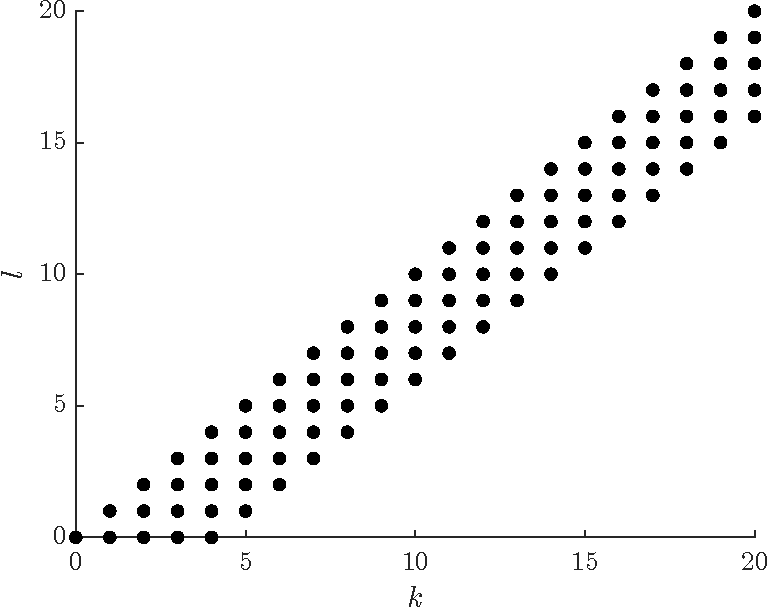
\includegraphics[width=0.5\textwidth]{supplements/ch1/ex1_17.pdf}
    \]
    Switching the order of summation therefore gives:
    \[
        B_n(x) =  \bsum[l] \sum_{k=l}^{l+n-1} b(n - 1, l)x^k = \bsum[l] \sum_{m=0}^{n-1} b(n - 1, l)x^{m+l}
    \]
    \[
        \Longleftrightarrow B_n(x) = \sum_{m=0}^{n-1} x^m \bsum[l] b(n - 1, l)x^l = (1+x+\ldots + x^{n-1})B_{n-1}(x)
    \]
    Because $B_1(x) = 1$ (there are no inversions), we find:
    \[
        B_n(x) = (1 + x)(1+x+x^2)\cdots(1+x+\ldots +x^{n-1})  
    \]
    For $n \leq 5$ we find:
    \begin{align*}
        B_1(x) &= 1 \\
        B_2(x) &= 1 + x \\
        B_3(x) &= 1 + 2x + 2x^2 + x^3 \\
        B_4(x) &= 1 + 3x + 5x^2 + 6x^3 + 5x^4 + 3x^5 + x^6 \\
        B_5(x) &= 1 + 4x + 9x^2 + 15x^3 + 20x^4 + 22x^5 + 20x^6 + 15x^7 + 9x^8 + 4x^9 + x^{10}
    \end{align*}
\end{solution}

\begin{exercise}
    \begin{enumerate}[label=(\alph*)]
        \item Given $n,k$. For how many of the permutations of $n$ letters is it true that their first $k$ values decrease?
        \item What is the average length of the decreasing sequence with which the values of a random $n$-permutation begin?
        \item If $f(n,k)$ is the number of permutations that have exactly $k$ ascending runs, find the Pascal-triangle-type recurrence satisfied by $f(n,k)$. They are called the Euler numbers. As an example, the permutation
        \[
            \begin{pmatrix}
                1 & 2 & 3 & 4 & 5 & 6 & 7 & 8 & 9 \\
                4 & 1 & 6 & 9 & 2 & 5 & 8 & 3 & 7
            \end{pmatrix}
        \]
        has $4$ such runs, namely $4,\ 1\ 6\ 9,\ 2\ 5\ 8$ and $3\ 7$.
    \end{enumerate}
\end{exercise}
\begin{solution}
    \begin{enumerate}[label=(\alph*)]
        \item There are $\binom{n}{k}$ ways to choose the first $k$ numbers. Now, arrange them in decreasing order (there is only one such way). The other $n-k$ values can be arranged in $(n-k)!$ ways, so there are 
        \[
            \binom{n}{k}(n-k)! = \frac{n!}{k!(n-k)!}(n-k)! = \frac{n!}{k!}
        \]
        where the first $k$ values decrease.
        \item Since there are $\frac{n!}{k!}$ permutations where the first $k$ values decrease, there are $\frac{n!}{k!} - \frac{n!}{(k+1)!}$ where the first $k$ values decrease followed by an increase. For $k=n$, there is only one sequence (namely the decreasing permutation). Let $l(k)$ be the sum of all lengths of decreasing sequences of length $k$, then its sum is given by
        \[
            \sum_{k=1}^n l(k) = n + \sum_{k=1}^{n-1} k\left(\frac{n!}{k!} - \frac{n!}{(k+1)!}\right) 
        \]
        Factoring out $n!$ yields
        \[
            \sum_{k=1}^n l(k) = n + n! \sum_{k=1}^{n-1} \left(\frac{k}{k!} - \frac{k}{(k+1)!}\right)
        \]
        The sum of the second term for one value of $k$ and the first term of the next value is equal to $- \frac{k}{(k+1)!} + \frac{k+1}{(k+1!)} = \frac{1}{(k+1)!}$:
        \[
            \sum_{k=1}^n l(k) = n + n!\left(\frac{1}{1!}-\frac{n-1}{n!} + \sum_{k=2}^{n-1} \frac{1}{k!}\right)
        \]
        The average length is found by dividing by the total number of permutations $n!$
        \[
            \mathbf{E}(l) = \frac{n}{n!} + 1 - \frac{n-1}{n!} + \sum_{k=2}^{n-1} \frac{1}{k!} = \sum_{k=1}^{n} \frac{1}{k!}
        \]
        which is approximately $e-1$.
        \item Divide the permutation in $n$ letters with $k$ runs in two piles: one where $n$ is at the end of an existing run, i.e.\ the number before $n$ is larger than the number after $n$. This can be thought of as appending $n$ to one of the $k$ runs for a permutation of size $n-1$. The second pile contains the ones where removing $n$ reduces the number of runs. These can be constructed from a permutation of size $n-1$ with $k-1$ runs and inserting in any of the $(n-1) - (k-1) + 1 = (n-k+1)$ locations which do not extend an existing run. We therefore have the recurrence
        \[
            f(n,k) = kf(n-1,k) + (n-k+1)f(n-1,k-1)
        \]
    \end{enumerate}
\end{solution}

\begin{exercise}
    Consider the $256$ possible sums of the form
    \begin{equation} \label{eq:1:19}
        \epsilon_1 + \epsilon_2 + 2 \epsilon_3 + 5 \epsilon_4 + 10 \epsilon_5 + 10 \epsilon_6 + 20\epsilon_7 + 50 \epsilon_8
    \end{equation}
    where each $\epsilon$ is $0$ or $1$.
    \begin{enumerate}[label=(\alph*)]
        \item For each integer $n$, let $C_n$ be the number of different sums that represent~$n$. Write the generating polynomial
        \[C_0 + C_1x + C_2x^2 + C_3x^3 + \cdots + C_{99}x^{99}\]
        as a product.
        \item Next, consider all the possible sums that are formed as in \eqref{eq:1:19}, where now the $\epsilon$ can have any of the three values $-1,0,1$. For each integer $n$, let $D_n$ be the number of different sums that represent $n$. Show that some integer $n$ is representable in at least $33$ different ways. Then write the generating function
        \[
            \sum_{n=-99}^{99} D_nx^n
        \]
        as a product.
        \item Generalize the results of parts (a) and (b) of this problem by replacing the particular set of weights by a general set and each $\epsilon$ to be $\pm 1$. Factor the polynomial that occurs.
        \item In the general case of part (c) of this problem, state precisely what all of the zeros of the generating polynomial are, and state precisely what the multiplicity of each of the zeros is, in terms of the set of weights.
    \end{enumerate}
\end{exercise}

\begin{solution}
    \begin{enumerate}[label=(\alph*)]
        \item Suppose we only consider one variable (for example $\alpha\epsilon_1$) then the generating polynomial is given by:
        \[
            (1+x^\alpha)
        \]
        since there are only two possibilities. Now summing two variables lead to the product of these components since all combinations are made. For example:
        \[
            (1+x^\alpha)(1+x^\beta) = (1 + x^\alpha + x^\beta + x^{\alpha+\beta})
        \]
        which is indeed the generating polynomial of the sum. The generating polynomial of $\{C_n\}$ is:
        \[
            (1+x)^2(1+x^2)(1+x^5)(1+x^{10})^2(1+x^{20})(1+x^{50})
        \]
        \item There are $3^8 = 6561$ possible combinations of all the $\epsilon$ values. All sums are between $-99$ and $99$. Thus there are $199$ possible sums. From the pigeonhole principle it follows that there is an integer $n$ which is representable in at least $\lceil \frac{6561}{199}\rceil = 33$ ways. The generating polynomial is found analogously with one of the `building blocks' equal to $(x^{-w} + 1 + x^w)$:
        \[
            (x^{-1}+1+x)^2 (x^{-2} + 1 + x^2)(x^{-5} + 1 + x^5)\cdots(x^{-50} + 1 + x^{50})
        \]
        \item Assume that the possible (distinct) weights are $w_1, w_2, \ldots, w_r$. Each factor has the form
        \[
            (x^{-w_i} + x^{w_i})
        \]
        such that the generating polynomial is:
        \[
            \infsum D_n x^n = \prod_{i=1}^r (x^{-w_i} + x^{w_i})
        \]
        \item The zeros are easily found from the factored representation. Each factor contributes $2w_i$ roots. Indeed:
        \[
            (x^{-w_i} + x^{w_i}) = 0 \Leftrightarrow x^{2w_i} = -1
        \]
        The roots are therefore the $2w_i$th roots of $-1$.
    \end{enumerate}
\end{solution}

\begin{exercise}
    Let $f(n,m,k)$ be the number of strings of $n$ $0$'s and $1$'s that contain exactly $m$ $1$'s, no $k$ of which are consecutive.
    \begin{enumerate}[label=(\alph*)]
        \item Find a recurrence formula for $f$. It should have $f(n,m,k)$ on the left side, and \textit{exactly three terms on the right}.
        \item Find, in simple closed form, the generating functions
        \[
            F_k(x,y) = \sum_{n,m\geq 0} f(n,m,k)x^ny^m \quad (k=1,2,\ldots)
        \]
        \item Find an explicit formula for $f(n,m,k)$ from the generating function (this should involve only a single summation, of an expression that involves a few factorials).
    \end{enumerate}
\end{exercise}

\begin{solution}
    \begin{enumerate}[label=(\alph*)]
        \item The last character of the string is either $0$ or $1$. This gives the first two terms of the recurrence relation:
        \[
            f(n,m,k) = f(n-1,m,k) + f(n-1,m-1,k) + \ldots
        \]
        where the first term corresponds to adding $0$ and the second term adds $1$. This however overcounts the number of strings since adding a $1$ may violate the restriction on the consecutive number of $1$'s. These correspond to the number of strings ending in $01^k$ appended to all strings of size $n-k-1$ ending with $m-k$ $1$'s and which do not violate the constraint. The recurrence relation is therefore:
        \[
            f(n,m,k) = f(n-1,m,k) + f(n-1,m-1,k) - f(n-k-1,m-k,k)
        \]
        thought it does not always hold as we will see later.

        Assume that $k \geq 2$ (or the restriction on $k$ does not make much sense). The base cases are as follows. For $n<0$ or $m<0$, $f(n,m,k) = 0$ since no string exists. Now check $(n,m) = (1,0)$:
        \[
            f(1,0,k) = f(0,0,k) + f(0,-1,k) - f(-k,-k,k) = f(0,0,k)
        \]
        but $f(1,0,k) = 1$ because only the singleton string $0$ is valid. Therefore $f(0,0,k) = 1$ is required. Notice that the recurrence relation does not hold for $(n,m) = (0,0)$ since 
        \[
            1 = f(0,0,k) = f(-1,0,k) + f(-1,-1,k) - f(-k-1,-k,k) = 0
        \]

        The other case for which the recurrence does not hold is due to the assumption that the end of the `violating' string is given by $01^k$. For $(n,m) = (k,k)$, the correction term should be $f(k-k,0,k) = 1$ instead of $f(k-k-1,0,k) = 0$ such that $f(k,k,k) = 0$ (no valid string).
        \item Multiplying both sides by $x^ny^m$ and summing over $n,m\geq 0$ except for $(n,m) = (0,0)$ and $(n,m) =(k,k)$ (these terms are added and subtracted so the definition of the generating function is found again, the resulting terms with negative $n$ or $m$ have already been omitted since they are $0$):
        \begin{align*}
            F_k - f(0,0,k) &= x(F_k - f(k-1,k,k)x^{k-1}y^k) + 
             xy(F_k - \\
            &\mspace{75mu} f(k-1,k-1,k)x^{k-1}y^{k-1}) - x^{k+1}y^k F_k
        \end{align*}
        As pointed out above $f(0,0,k) = 1$. $f(k-1,k,k) = 0$ since no string of length $k-1$ can have $k$ $1$'s. $f(k-1,k-1,k) = 1$ since only the string of only $1$'s is valid:
        \[
            F_k - 1 = xF_k + xy(F_k - x^{k-1}y^{k-1}) - x^{k+1}y^kF_k
        \]
        Solving for $F_k$ gives:
        \[
            F_k(x,y) = \frac{1-x^ky^k}{1-x-xy+x^{k+1}y^k}
        \]
        \item An explicit formula for $f(n,m,k)$ can be found by extracting the coefficent:
        \[
            f(n,m,k) = \coeff{x^ny^m} \frac{1-x^ky^k}{1-x-xy+x^{k+1}y^k}
        \]
        Isolating $(1-xy)$ in the denominator:
        \[
            f(n,m,k) = \coeff{x^ny^m} \frac{1-x^ky^k}{1-xy}\frac{1}{1 - x\frac{1 - x^ky^k}{1-xy}}
        \]
        Expanding the geometric series \eqref{eq:power_geom}:
        \begin{align*}
            f(n,m,k) &= \coeff{x^ny^m} \frac{1-x^ky^k}{1-xy} \bsum[l] \left(\frac{1-x^ky^k}{1-xy}\right)^l x^l \\
            &= \coeff{x^ny^m} \bsum[l] \left(\frac{1-x^ky^k}{1-xy}\right)^{l+1} x^l 
        \end{align*}
        Using the binomial expansions \eqref{eq:binom_num}, \eqref{eq:binom_denom}:
        \[
            f(n,m,k) = \coeff{x^ny^m} \bsum[l]\infsum[i]\infsum[j] (-1)^{i}\binom{l+1}{i}\binom{j+l}{j} x^{ik+j+l}y^{ik+j}
        \]
        Using $m=ik+j$ to eliminate $j= m - ik$:
        \[
            f(n,m,k) = \coeff{x^n} \bsum[l]\infsum[i] (-1)^i \binom{l+1}{i} \binom{m-ik+l}{m-ik}x^{m+l}
        \]
        Letting $n=m+l$ to eliminate $l=n-m$ yields the final formula for $n\geq m$
        \[
            f(n,m,k) = \infsum[i](-1)^i\binom{n-m+1}{i}\binom{n-ik}{m-ik}
        \]
    \end{enumerate}
\end{solution}

\begin{exercise}
    \begin{enumerate}[label=(\alph*)]
        \item We want to find a formula for the $n$th derivative of the function $e^{e^x}$. Differentiate it a few times, study the pattern, and conjecture the form of the answer for general $n$, including some constants to be determined. Then find a recurrence formula for the constants in question, and identify them as some `famous' numbers that we have studied.
        \item Next let $f(x_1,\ldots,x_n)$ be some function of $n$ variables. Find a formula for the mixed partial derivative 
        \[
            \frac{\partial^n}{\partial x_1\partial x_2\cdots\partial x_n}e^f
        \]
        that expresses it in terms of various partial derivatives of $f$ itself.
    \end{enumerate}
\end{exercise}

\begin{solution}
    \begin{enumerate}[label=(\alph*)]
        \item Differentiating $e^{e^x}$ a few times:
        \begin{align*}
            De^{e^x} &= e^{e^x}e^x \\
            D^2e^{e^x} &= e^{e^x}(e^{2x} + e^x) \\
            D^3e^{e^x} &= e^{e^x}(e^{3x} + e^{2x} + 2e^{2x} + e^x) \\
            &= e^{e^x}(e^{3x} + 3e^{2x} + e^x) \\
            D^4e^{e^x} &= e^{e^x}(e^{4x} + 3e^{3x} + e^{2x} + 3e^{3x} + 6e^{2x} + e^x) \\
            &= e^{e^x}(e^{4x} + 6e^{3x} + 7e^{2x} + e^x) \\
            D^ne^{e^x} &= e^{e^x}(c_ne^{nx} + c_{n-1}e^{(n-1)x} + \ldots + c_{1}e^{x})
        \end{align*}
        Denote the constant corresponding to $e^{kx}$ in the $n$th derivative as $\stirlingSnd{n}{k}$. Then it will satisfy the recurrence relation:
        \[
            \stirlingSnd{n}{k} = \stirlingSnd{n-1}{k-1} + k \stirlingSnd{n-1}{k}
        \]
        The first term comes from differentiating $e^{e^x}$ and multiplying with the term $e^{(k-1)x}$. The second term follows from differentiating $e^{kx}$.

        The base case is $\stirlingSnd{0}{0} = 1$ since the zeroth derivative is $e^{e^x}$ itself. This is exactly the same recurrence relation as the Stirling numbers of the second kind.
        \item Again writing the derivatives for $n=1,2,\ldots$:
        \begin{align*}
            \frac{\partial}{\partial x_1}e^f &= e^f\frac{\partial f}{\partial x_1} \\
            \frac{\partial^2}{\partial x_1 \partial x_2}e^f &= e^f\left(\frac{\partial f}{\partial x_2}\frac{\partial f}{\partial x_1} + \frac{\partial^2 f}{\partial x_1 \partial x_2}\right) \\
            \frac{\partial^3}{\partial x_1 \partial x_2 \partial x_3}e^f &= e^f\left(\frac{\partial f}{\partial x_3}\frac{\partial f}{\partial x_2}\frac{\partial f}{\partial x_1} + \frac{\partial f}{\partial x_3}\frac{\partial^2 f}{\partial x_1 \partial x_2} + \right. \\
            & \mspace{60mu} \left.\frac{\partial^2 f}{\partial x_3 x_2}\frac{\partial f}{\partial x_1} + \frac{\partial f}{\partial x_2}\frac{\partial^2 f}{\partial x_3 x_1} + \frac{\partial^3 f}{\partial x_1 \partial x_2 \partial x_3} \right)
        \end{align*}
        Every partition of $[n]$ has a term in the mixed partial derivative. The mixed partial derviative of order $n$ is therefore:
        \[
            \frac{\partial^n}{\partial x_1\partial x_2\cdots\partial x_n}e^f = e^f\left(\sum_{\pi_i\in\pi} \prod_{B \in \pi_i} \frac{\partial^{|B|}f}{\prod_{j\in B} \partial x_j}\right)
        \]
        where $\pi$ is the set of all partitions, $B$ loops over all classes of each partition and $j$ loops over the elements in the class. This is seen inductively from the construction of the set of partitions of $[n]$ from the partitions of $[n-1]$.

        Indeed, suppose the formula holds for $n-1$ and consider differentiating with respect to $x_n$. From the product rule, first differentiating $e^f$ and multiplying with the second term gives rise to partitions where $n$ is in its own class. Further, differentiating the class from each partition of $[n-1]$ corresponds to applying the product rule where each term is adding $n$ to the $i$th class.
    \end{enumerate}
\end{solution}